	\documentclass[../pfc.tex]{subfiles}

	
	\begin{document}
	
La fase de análisis y el proceso de Ingeniería de Requisitos, parten básicamente de dos contextos bien diferenciados:\\
-Por una parte de las reuniones mantenidas con el cliente, en este caso la AECC.

-Por otra parte del libro que utiliza la AECC llamado \textbf{MIS CUIDADOS, DIARIO DE SALUD DE UN SUPERVIVIENTE DE CANCER} y que se utiliza de manera general sobre enfermos de cáncer que han superado esta enfermedad y sobre otros que todavía la siguen padeciendo.\\\\
	
	\section{¿El porqué?}
	
	Desde el punto de vista de la definición clásica:
	
	La ingeniería del software es el proceso formal de desarrollo de software en el que las necesidades del usuario se traducen en requisitos, estos se transforman en diseño que se implementa en código que se prueba, documenta y se certifica para su uso operativo. Según la definición del IEEE la ingeniería del software se define como “(1) la aplicación de un método sistemático, disciplinado y cuantificable al desarrollo, operación y mantenimiento de software, esto es, la aplicación de la ingeniería al software” y “(2) el estudio de los métodos de (1)”\\
	
	El proceso requiere una metodología con 5 etapas:
	
	Análisis de requisitos: Se extraen los requisitos del producto de software. En esta etapa la habilidad y experiencia en la ingeniería del software es crítica para reconocer requisitos incompletos, ambiguos o contradictorios.\\
	Usualmente el cliente/usuario tiene una visión incompleta/inexacta de lo que necesita y es necesario ayudarle para obtener la visión completa de los requerimientos.  El contenido de comunicación en esta etapa es muy intenso ya que el objetivo es eliminar la ambigüedad en la medida de lo posible.\\
	Partiendo de un exhaustivo estudio de las funcionalidades que podrian resultar útiles para los pacientes de Cancer, y de acuerdo con las especificaciones de la AECC hemos decidido incluir en la misma las siguientes:\\

	
	AVATAR -> 		Editar el perfil, Foto, nombre, apellidos, edad, cumpleaños... (1 pantalla), ¿Grupo sanguineo y alergenos tampoco estaría mal pero es informacion de otro nivel LOPD?
	PROYECTO AMPLIACION (asignar un agente personalizado para poder atender de manera personalizada al paciente Superviviente)
	
	PRINCIPAL-> 	Vista de Rutina proxima, citas, Se debería ver lo que realmente interesa ¿Noticias AECC tipo RSS, Twitter, Facebook? (1 pantalla)
	
	HORARIO -> 		Vista dia, mes, con las actividades, citas, ¿Cumpleaños, aniverssario de enfermedad...?  
	al pinchar en una hora, dia, se podrá añadir rutina o cita, iria a la correspondiente lista de creacion de una nueva (1 pantalla)
	Deberian aparecer las citas y rutinas ocupando el espacio destinado a la duracion de las mismas.
	Revisar esta página
	https://code.google.com/p/yadview/
	
	RUTINA -> 		Lista de rutinas,
	Desde la propia vista se podrán añadir rutinas, al pulsar sobre la opción correspondiente nos llevará al listado de estás opciones añadiendose así.
	Se podra ordenar por fecha, asc y desc, duracion de la actividad asc y desc pero sobre todo se podrá ordenar por satisfaccion de la misma.
	
	
	Añadir rutina, , en esta pantalla se permite ver al pinchar sobre el propio item de la lista ,editar, o pulsando el botón añadir del final de la lista crear una nueva,
	Valorar si deberiamos gestionar la repeticion de los elementos					
	dentro de la rutina (añadir) se podrán añadir personajes y asignar una alarma personalizable (avisar) con antelacion, se puede ver sin editar(2 pantallas)
	con una hora de aviso, hora de empiece de la actividad. Duración de las misma en horas, satisfaccion de 0 a 10
	Dentro se va a valorar tambien la satisfacción personal que se produce al hacer esto, podrá ser de 0 a 10
	
	AMPLIACION DE PROYECTO: Poder variar los avisos para que se hagan de manera repetitiva, por ejemplo repetir de manera semanal los jueves al estilo TICK TICK, llamarlo actividades en vez de Rutina 
	
	CITAS -> 		Lista de citas Nombre de la cita, fecha y hora.
	Desde el propio item de la lista se podran añadir medicamentos, personas, sintomas y/o pruebas, al pulsar sobre la opción correspondiente nos llevará al listado de estás opciones añadiendose así.
	
	Añadir cita, en esta pantalla se permite ver al pinchar sobre el propio item de la lista ,editar, o pulsando el botón añadir del final de la lista crear una nueva, 
	dentro de la cita (añadir) se podrán añadir ubicación, personajes, medicamentos, pruebas y sintomas y asignar una alarma personalizable con fecha y hora (avisar) con antelacion.
	se puede ver sin editar
	Deberíamos añadir duración?
	Valorar si deberiamos gestionar la repeticion de los eventos
	¿En la ubicación se podria comunicar con google maps?
	¿Deberiamos mostrar en el item de la cita si ya poseee personas, pruebas, sintomas o medicacion?
	
	PROYECTO AMPLIACION Poder exportar e importar a google maps, conectar la ubicacion con google maps para poder ir
	
	MEDICACION -> 	Lista de medicamentos, lista de los medicamentos que tengamos con el boton de añadir al final y en la barra la posibilidad de ordenar en principio por orden ascendente o descendente,
	al pinchar sobre el elemento se visualiza, 
	en las opciones de cada elemento se puede añadir a la cita, editar y borrar (confirmacion para borrar)
	
	Añadir medicamento, , en esta pantalla se permite ver al pinchar sobre el propio item de la lista ,editar, o pulsando el botón añadir del final de la lista crear una nueva, 
	dentro del medicamento (añadir) se podrá asignar una foto personalizable, o bien hacerla o añadirla de la galeria, viene una por defecto
	nombre, descripcion, 
	una alarma personalizable que avisar con antelacion, fecha inicio, hora inicio, fecha fin, hora fin, repetir cada tantas horas, dias, semanas, (esto se valorará)
	REVISAR LA FUNCION DE ALARMA EN ANDROID http://developer.android.com/reference/android/app/AlarmManager.html
	boton guardar 
	se puede ver sin editar, 
	dentro de la edición y visionado se podra añadir a una cita
	Se puede añadir el numero de medicamentos al drawer (se estudiará)
	
	PROYECTO AMPLIACION Llevar el stock de lo que lleva consumido el paciente y generar alertas para cuando se le acabe, duplicar tratamiento, para ahorrar trabajo, opciones de dosis.
	
	PERSONAJES -> 	Lista de personajes que tengamos con el boton de añadir al final y en la barra la posibilidad de ordenar en principio por orden ascendente o descendente,
	al pinchar sobre el elemento se visualiza, 
	en las opciones de cada elemento se puede añadir a la cita, a la rutina, editar y borrar confirmacion para borrar
	
	Añadir persona, , en esta pantalla se permite ver al pinchar sobre el propio item de la lista ,editar, o pulsando el botón añadir del final de la lista crear una nueva, 
	dentro de la persona(añadir) se podrá asignar una foto personalizable, o bien hacerla o añadirla de la galeria, viene una por defecto
	nombre apellidos, puesto / tipo (doctor, oncologo, cirujano, farmaceutico, enfermero, medico cabecera, familiar, amigo,AECC, otro), telefono (posibilidad de llamar desde la visualizacion)
	se puede ver sin editar, dentro de la edición y visionado se podra añadir a una cita, o a una rutina ejemplo (paseo por la playa) o a cita con el oncólogo
	Se puede añadir el numero al drawer
	
	PROYECTO AMPLIACION llevarnos ese contacto a la agenda o traernosle de ella
	
	PRUEBAS -> 	 	Lista de personajes que tengamos con el boton de añadir al final y en la barra la posibilidad de ordenar en principio por orden de fecha ascendente o descendente,
	al pinchar sobre el elemento se visualiza, 
	en las opciones de cada elemento se puede añadir a la cita, editar y borrar confirmacion para borrar
	
	Añadir prueba, , en esta pantalla se permite ver al pinchar sobre el propio item de la lista ,editar, o pulsando el botón añadir del final de la lista crear una nueva, 
	dentro de la prueba (añadir) se podrá asignar una foto personalizable, o bien hacerla o añadirla de la galeria, viene una por defecto
	nombre, descripcion,
	fecha y hora de la misma
	se puede ver sin editar, dentro de la edición y visionado se podra añadir a una cita por ejemplo visita al oncólogo
	Se puede añadir el numero al drawer
	
	PROYECTO AMPLIACION poder subir documentos tipo pdf para no depender de la fotografia solo, llevar estadísticas
	
	SINTOMAS ->  	Lista de síntomas que tengamos con el boton de añadir al final y en la barra la posibilidad de ordenar en principio por orden de fecha ascendente o descendente,
	al pinchar sobre el elemento se visualiza, 
	en las opciones de cada elemento se puede añadir a la cita, editar y borrar confirmacion para borrar
	
	Añadir sintoma, , en esta pantalla se permite ver al pinchar sobre el propio item de la lista ,editar, o pulsando el botón añadir del final de la lista crear una nueva, 
	dentro de la prueba (añadir) se podrá asignar una foto personalizable, o bien hacerla o añadirla de la galeria, viene una por defecto
	nombre, descripcion de los sintomas,
	fecha y hora de la misma
	se puede ver sin editar, dentro de la edición y visionado se podra añadir a una cita por ejemplo visita al oncólogo
	Se puede añadir el numero al drawer
	
	PROYECTO AMPLIACION poder subir documentos tipo pdf para no depender de la fotografia solo, llevar estadísticas, poder conectar con los centros de salud, hospitales, 
	
	RECURSOS  -> 	Dentro de los resursos aparece meditacion con musica relajante e instrucciones para ello
	consejos generales, de alimentacion, de vida, de salud...
	telefonos de interés generales (DEBEMOS DECIDIR SI SE PUEDEN PERSONALIZAR)
	Noticias (podemos añadir el blog de la AECC o la cuenta de twitter que no esta nada mal)
	
	AJUSTES  ->  	Editar el perfil, 
	tamaño de letra, 	
	tono para alertas de citas y rutinas, 
	color del led de notificación, 
	posibilidad de feedback,
	quienes somos o motivaciones (¿? pantallas)
	NO VOY A AÑADIR MÁS PANTALLAS AL RESPECTO, SE HABLARÁ
	
	\section{Documento de Análisis}
	
	Aunque utilizamos una metología ágil, hay puntos en los que no nos podemos separar de la metodología tradicional.
			
	Es difícil capturar todos los requisitos a partir de unas cuantas reuniones, para nuestro caso, pudimos contar con la ayuda del libro "Mis Cuidados, diario de salud para supervivientes de cáncer"
			
	Una de las ventajas de utilizar este primer tipo de metodología, es el de poder adaptar de una manera mucho más eficiente los recursos a las fechas y a los requisitos, y poder modificar estos requisitos de manera "ágil" debido al panorama cambiante que podemos tener de cara al cliente.
			
	\begin{figure}
		\centering
		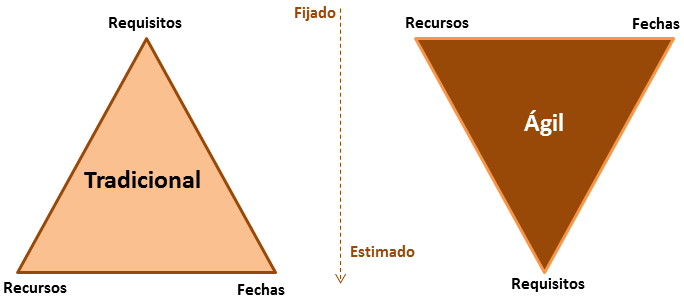
\includegraphics[width=0.5\linewidth]{../images/paradigmaRequisitos}
		\caption{Paradigma captura de requisitos método tradicional vs. ágil}
		\label{fig:paradigmaRequisitos}
	\end{figure}
			
			
			\subsection{Descripción de objetivos de manera detallada}
	
	\subsection{Captura de Requisitos}
	
	\subsubsection{Requisitos de información}
			
	
	\subsubsection{Requisitos Funcionales}
			
			

	\subsubsection{Requisitos No Funcionales}
	
	\subsection{Identificación de actores}
		
	\subsection{Diagrama de casos de uso }
		
	\subsection{Descripción de Casos de Uso}
		
	\subsection{Diagrama de clases de análisis}
		
	\subsection{Diagrama Entidad-Relación de la base de datos}
		
	\subsection{Modelo relacional del análisis}
	
\end{document}